\documentclass[hyperref={pdfpagelabels=false}]{beamer}
\usepackage{beamerthemesplit}
\usepackage[utf8]{inputenc}
\usepackage[T1]{fontenc}
\usepackage{lmodern}
\usepackage{graphicx}
\usepackage{amsmath, amsfonts, amssymb}
\usepackage{tikz}

\usetheme{Green}

\begin{document}
  \title{CoqOfOCaml}
  \author{Guillaume Claret}
  \date{5 September 2014}
  \maketitle

  \section{Introduction}
  \begin{frame}
    \frametitle{Two languages}
    \emph{OCaml}:
    \begin{itemize}
      \item programming language
      \item functional programming with imperative features
      \item many libraries and programs
    \end{itemize}
    \emph{Coq}:
    \begin{itemize}
      \item (mainly used as a) proof language
      \item purely functional programming (not even non-termination)
      \item limited number of libraries for the programmer
    \end{itemize}
  \end{frame}
  \begin{frame}
    \frametitle{Bridges}
    \emph{Coq} to \emph{OCaml}: extraction mechanism:
    \begin{itemize}
      \item developed mainly by Pierre Letouzey
      \item removes the proof terms
      \item converts the remaining purely functional expressions to \emph{OCaml}
      \item complete
    \end{itemize}
    \emph{OCaml} to \emph{Coq}:
    \begin{itemize}
      \item \emph{CFML}: deep embedding
      \item how to do shallow embedding?
      \item how to import imperative programs?
    \end{itemize}
  \end{frame}
  \begin{frame}
    \frametitle{CopOfOCaml}
    \begin{center}
      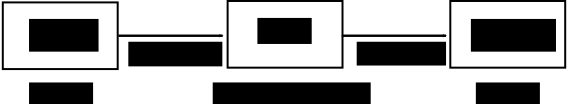
\includegraphics[width=10cm]{images/compilation_chain}
    \end{center}
    We use a \emph{monadic translation} to represent imperative features in~\emph{Coq}.
  \end{frame}
  \begin{frame}
    \frametitle{Usages}
    You may want to:
    \begin{itemize}
      \item prove formal properties on \emph{OCaml} programs
      \item augment the number of \emph{Coq} libraries for programming
    \end{itemize}
  \end{frame}
  \begin{frame}
    \frametitle{Informal specification}
    The following programs are equivalent (same input-output traces):
    \begin{itemize}
      \item \texttt{foo.ml} and \texttt{foo.v} (interpreting the monad)
      \item \texttt{foo.v} and \texttt{foo2.ml}
    \end{itemize}
    Not proved.
  \end{frame}
  \begin{frame}
    \frametitle{Quick demo}
    {\Huge Quick demo.}
  \end{frame}
\end{document}